\chapter{Game Attributes}

\section{Hero Details}
We have four heroes to play with as shown in Figure 6.\\

\begin{figure}[htp]
\centering
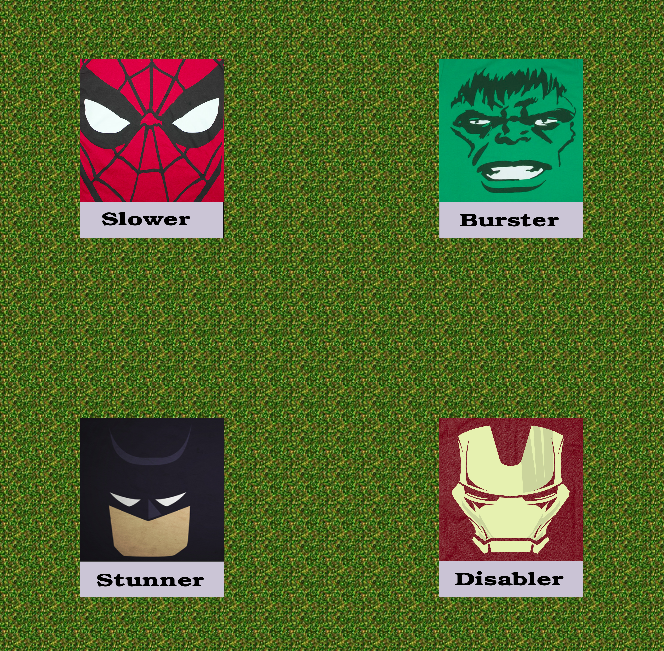
\includegraphics[width=0.5\textwidth]{Heros.png}
\caption{\label{fig:heroes}Heroes}
\end{figure}

Each hero has a unique magic power as described:
\begin{enumerate}
\item Stunner: Freezes the enemy player from attacking, moving, etc. for few seconds.
\item Slower: Reduces the attack capability of the enemy player for few seconds.
\item Disabler: Disables the enemy player from using any magical power for few seconds.
\item Burster: Does burst damage in a single shot.
\end{enumerate}

A hero is not allowed to use magic power in succession. It has to wait for some time before it can re-use the magic. \\

When a player uses it’s magic power on an enemy player, the enemy player is said to be cursed.

\section{Game Stats}
Each temple’s initial health is 500. Each hero’s initial heath is 200.
\\ \\
A hero has following attributes besides it’s health:
\begin{enumerate}
\item Strength: Damage done on a single attack
\item Speed: Movement speed (MIN 0 MAX 5)
\end{enumerate}

The above attributes depend on the hero type, as follows:
\begin{enumerate}
\item Stunner: Strength - 4, Speed - 2
\item Slower: Strength - 5, Speed - 2
\item Disabler: Strength - 6, Speed - 3
\item Burster: Strength - 7, Speed - 2
\end{enumerate}



\section{Item Details}
We have four items in our game. These items add to certain capabilities of the hero.
\begin{enumerate}
\item Speed Gain: Increases movement speed of the player by 1.
\item Strength Gain: Increases damage capability of the player by 2.
\item Temple Healer: Increases health of the player’s temple by 50.
\item Heath Gain: Increases health of the player by 20.
\end{enumerate}

